\documentclass{article}
\usepackage{graphicx}
\usepackage{makecell}
\usepackage[T1]{fontenc}
%\usepackage{tgpagella}      
\usepackage[dvipsnames]{xcolor}
\usepackage{booktabs}
\usepackage{comment}
\usepackage{longtable}
\usepackage{tgpagella} 
\usepackage{xfrac} 
\usepackage{float} 
\usepackage{colortbl}
\usepackage{hyperref}
%\RequirePackage{fontawesome}

\hypersetup{
    colorlinks=true, 
    linktoc=all,     
    linkcolor=black!80,
}
\renewcommand{\arraystretch}{1.4}
\newcommand{\must}{\cellcolor{Green}{M}}
\newcommand{\should}{\cellcolor{LimeGreen}{S}}
\newcommand{\could}{\cellcolor{RedOrange}{C}}
\newcommand{\wont}{\cellcolor{BrickRed}{W}}

\title{\huge Gestione del Progetto}
\author{Gabriele Chignoli}
\date{Maggio 2025}
\begin{document}
\maketitle
\newpage
\tableofcontents
\newpage

\section{Ciclo di Vita del Software}
Dopo un'analisi dei principali modelli disponibili per la modellazione del ciclo di vita del software, si è giunti alla conclusione che sia gli approcci "pesanti" che quelli più agili hanno utili proprietà che vanno combinate per portare ad un processo più, secondo il team, completo e "umano".  \newline 

Dei processi pesanti, viene considerata la pianificazione iniziale fondamentale a garantire che il progetto mantenga nel tempo dei binari definiti entro cui operare. Tuttavia, si considera che tale processo rischi di diventare troppo morboso, e l'impossibilità di tornare ad operare su fasi iniziali già completate, viene vista come una grande limitazione. 

Per questi motivi è stato deciso di adottare il \textbf{Modello a Cascata} come modello base per la produzione del progetto; di questo, si intende poter "risalire la cascata" ogni qualvolta sia necessario (credendo nel fatto che le risalite diminuiscano con l'avanzamento del progetto), risultando così in parte simile ad un approccio evolutivo, senza tuttavia l'obbligo di eseguire tutte le fasi ad ogni ciclo. Infine, si considerano le tre fasi finali di implementazione, testing e manutenzione come un processo continuo in cui ogni parte è fondamentale per la seguente, e necessita di quella che l'ha preceduta. Dunque si ritiene che una visione più ciclica di tali fasi sia più adatta. \newline 

Tenendo in mente queste accortezze, si è tentato di rappresentare anche graficamente il modello adottato:

\begin{figure}[H]
    \centering
    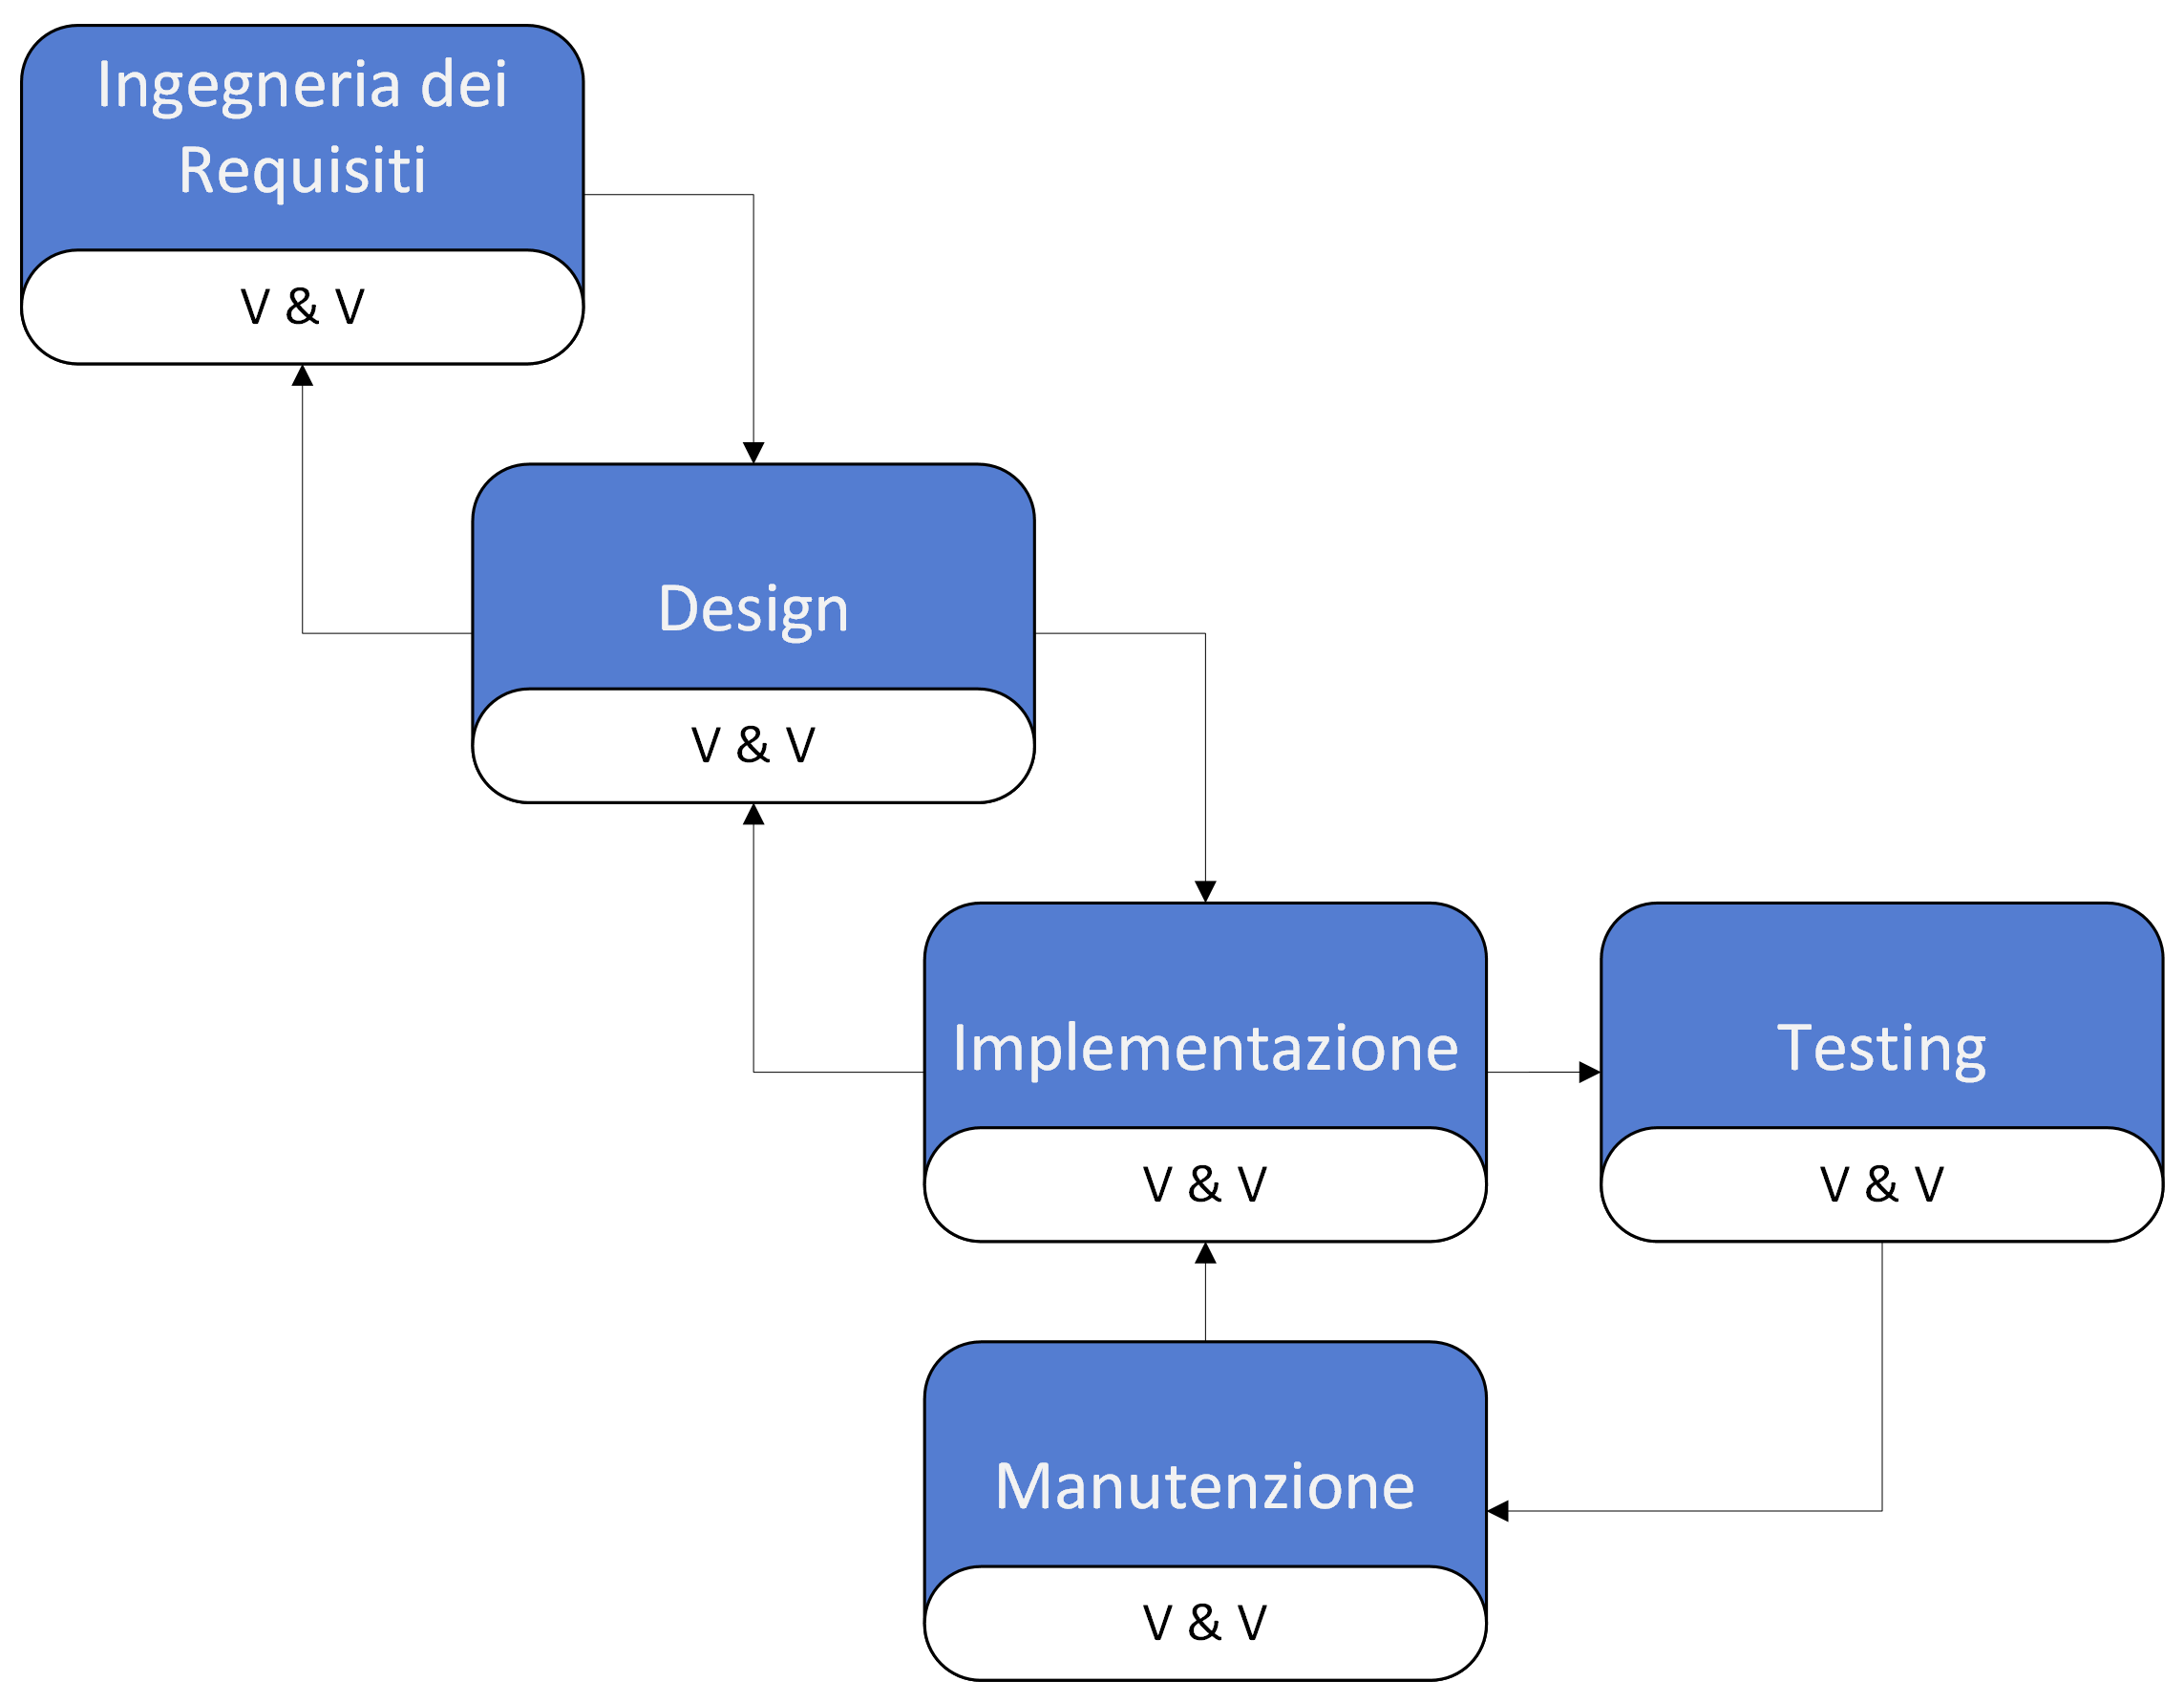
\includegraphics[width=.8\linewidth]{imgs/Modello a Cascata_0.png}
    \caption{Modello a Cascata Modificato}
    \label{fig:enter-label}
\end{figure}



\section{Configuration Management}
Il progetto utilizza per la gestione della configurazione la piattaforma \textbf{\textit{GitHub}}, del quale si intendono utilizzare le principali funzionalità. Inoltre si utilizzerà la \textbf{\textit{Kanban Board} }messa a disposizione nella sezione \textit{Progetti} di \textit{GitHub}, con la quale tenere traccia dei compiti e del loro stato. 

\section{People Management}
Pur essendo composto attualmente da un solo membro, si considera comunque di valore stabilire un'organizzazione del team secondo la quale si intende operare. Date le dimensioni del progetto abbastanza contenute e il tipo di personale disponibile (studenti universitari), si ritiene che la struttura più adatta per lo svolgimento del compito sia un'\textbf{Organizzazione a Matrice}. 

In tal modo, tutti i membri possono operare su diverse (anche tutte) parti del progetto e quindi imparare, facendo, come costruire un software nella sua completezza, dalla documentazione e progettazione, al testing e all'implementazione, sfruttando questo ambiente "sandbox", invece che avere effettive responsabilità come nel mondo lavorativo. \newline 

Le principali aree di lavoro e la loro allocazione al personale attuale (24/05/2025) sono elencate nella seguente tabella:
\begin{center}
    \begin{longtable}{ccc}
    \toprule
         %\rowcolor{NavyBlue!70}
         \textbf{Area di Lavoro} & \textbf{Personale}  & \\
         \midrule
         & Gabriele Chignoli & \dots \\
    \midrule
         Documentazione & $100\%$  & \dots \\
         Interfaccia Grafica & $100\%$ & \dots  \\
         Logica dell'applicazione & $100\%$ & \dots \\
         Testing & $100\%$  & \dots \\
         Data Base & $100\%$  & \dots \\
         Manutenzione & $100\%$ & \dots  \\
    \bottomrule
    \end{longtable}
\end{center}

Nel casi si osservi, a fine progetto, che le percentuali effettive siano differenti da quelle previste, verrà allegata anche la versione con i dati effettivi. 

\end{document}
